\newpage
%
% Začiatok analýzy
% Úvod do analýzy
%
\ifthenelse {\boolean{bachelor}}
{
	%\section{Analysis}
	\section{Spracovanie prirodzeného jazyka} 
}
{
	%\chapter{Analysis}
	\chapter{Spracovanie prirodzeného jazyka}
}
V kapitole~\fullref{subsec:nlp} približujeme a rozoberáme spracovanie prirodzeného jazyka, jeho využitie v aplikáciach a systémoch a jeho hlavné úlohy. Ďalej v kapitole~\fullref{subsec:nlp_nastroje} analyzujeme nástroje, ktoré sa dajú využiť pri spracovávaní prirodzeného jazyka.

%
% Spracovanie prirodzeného jazyka
%
\ifthenelse {\boolean{bachelor}}
{
	%\subsection{Subsection}
	\subsection{Spracovanie prirodzeného jazyka}
}
{
	%\section{Subsection}
	\section{Spracovanie prirodzeného jazyka}
}
\label{subsec:nlp}
Spracovanie prirodzeného jazyka (angl. Natural Language Processing - NLP) odkazuje na počítačové systémy, ktoré spracovávajú, snažia sa pochopiť alebo generujú jeden alebo viacero ľudských jazykov. Vstupom môže byť text alebo hovorená reč s cieľom prekladu do iného jazyka, pochopenie a reprezentácia obsahu textu, udržanie dialógu s používateľom a iné~\cite{AllenNLP}. Počítače doposiaľ nedokážu plne porozumieť ľudskému jazyku, či už sa jedná o písaný alebo hovorený, a preto hlavným cieľom spracovania prirodzeného jazyka je vybudovať výpočtové modely prirodzeného jazyka pre jeho analýzu a generovanie~\cite{Bharati1995}.

Porozumenie ľudskej reči je mnohokrát náročné aj pre samotných ľudí a nie to ešte pre počítače. Na svete je veľké množstvo jazykov, ktoré sa od seba líšia charakteristikami typickými pre konkrétny jazyk. Navyše, každý človek je odlišný a typický, čo spôsobuje, že výslovnosť rovnakého slova viacerými ľuďmi môže byť odlišná. Ďalej máme slangové slová a slová typické len pre určité územie. Pri spracovávaní prirodzeného jazyka treba vziať do úvahy viaceré aspekty. Dosiahnutie tohto cieľa je preto často veľmi náročné.

V súčastnosti najpoužívanejšie algoritmy na spracovanie prirodzeného jazyka využívajú strojové učenie.
% Dosiahnutie úplného porozumenia a spracovania ľudského prirodzeného jazyka by znamenalo vyriešiť \textit{AI-complete} problém, čo znamená, že obtiažnosť tohto problému je ekvivalentná s obtiažnosťou problému vytvorenia počítača inteligentného ako človek, takzvané ,,true AI''.


%
% Úlohy spracovania prirodzeného jazyka
%
\ifthenelse {\boolean{bachelor}}
{
	%\subsection{Subsection}
	\subsection{Úlohy spracovania prirodzeného jazyka}
}
{
	%\section{Subsection}
	\subsection{Úlohy spracovania prirodzeného jazyka}
}
\label{subsec:tasksofnlp}
Spracovanie prirodzeného jazyka má niekoľko hlavných úloh. V nasledujúcich častiach sú podrobnejšie opísané tie, ktoré sú relevantné vzhľadom na spracovanie učebných textov.
Úlohy spracovania prirodzeného jazyka:~\cite{collobert2011} 
\begin{my_itemize}
	\myitem Značkovanie slovných druhov (angl. Part-of-speech tagging) \ref{subsubsec:postagging},
	\myitem Rozdelenie vety na menšie časti (angl. Chunking),
	\myitem Rozpoznávanie názvoslovných entít (angl. Named Entity Recognition) \ref{subsubsec:ner},
	\myitem Označovanie sémantického postavenie (angl. Semantic Role Labeling),
	\myitem Rozpoznanie koreferencií (angl. Coreference resolution) \ref{subsubsec:corefparsing},
	\myitem Morfologické segmentovanie (angl. Morphological Segmentation),
	\myitem Generovanie prirodzeného jazyka (angl. Natural Language Generation),
	\myitem Optické rozoznávanie textu (angl. Optical Character Recognition),
	\myitem Rozloženie vzťahov (angl. Dependency parsing) \ref{subsubsec:dependencyparsing},
	\myitem a ďalšie.
\end{my_itemize}

Hlavné úlohy spracovania prirodzeného jazyka sú implementované a využívané vo viacerých smeroch. Z hľadiska spracovania učebných textov je pre nás najdôležitejšie využitie extrakcie informácií, ktoré je podrobnejšie popísané v sekcii~\fullref{subsubsec:information_extraction}. Ďalšie využitia spracovania prirodzeného jazyka sú napríklad:~\cite{Preeti}
\begin{my_itemize}
	\myitem strojový preklad (angl. Machine Translation),
	\myitem rozpoznávanie reči (angl. Speech Recognition),
	\myitem sumarizáciu textu (angl. Text Summarization),
	\myitem dialógové systémy (angl. Dialogue Systems),
	\myitem vyhľadávanie informácií (angl. Information Retrieval),
	\myitem a ďalšie.
\end{my_itemize}

%
% Značkovanie slovných druhov
%
\ifthenelse {\boolean{bachelor}}
{
	%\subsection{Subsection}
	\subsubsection{Značkovanie slovných druhov}
}
{
	%\section{Subsection}
	\subsection{Značkovanie slovných druhov}
}
\label{subsubsec:postagging}
Hlavnou úlohou značkovania slovných druhov (angl. Part-of-speech tagging) je každému slovu vo vete priradiť unikátnu značku označujúcu jeho syntaktickú úlohu vo vete~\cite{collobert2011}. Sú to, napríklad v slovenskom jazyku podmet, prísudok, príslovkové určenie alebo v anglickom jazyku noun, adverb, verb, atď. Okrem vymenovaných označení to môže byť aj označenie určujúce množné číslo, napríklad singulár alebo plurál.

Problémom pri značkovaní slovných druhov je mnohoznačnosť. Mnohoznačnosť je vlastnosť slova spôsobujúca, že slovo môže mať viacero významov a môže byť viacerými slovnými druhmi. V slovenskom jazyku napríklad slovo \textit{kry} môže predstavovať sloveso s významom rozkazu \textit{prikry!}, ale taktiež môže predstavovať podstatné meno s významom \textit{kríky}. V anglickom jazyku napríklad slovo \textit{book}, ktoré môže predstavovať podstatné meno \textit{kniha} alebo sloveso vo význame \textit{rezervovať}.

%
% Rozpoznávanie názvoslovných entít
%
\ifthenelse {\boolean{bachelor}}
{
	%\subsection{Subsection}
	\subsubsection{Rozpoznávanie názvoslovných entít}
}
{
	%\section{Subsection}
	\subsection{Rozpoznávanie názvoslovných entít}
}
\label{subsubsec:ner}
Rozpoznávanie názvoslovných entít (angl. Named Entity Recognition) označuje mená a názvy (entity), ktoré sa vyskytujú v texte. Tie následne rozdeľuje do kategórií, ako sú napríklad \textit{osoby}, \textit{organizácie} alebo \textit{lokácie}~\cite{collobert2011}.

Ťažkosti pri rozpoznávaní názvoslovných entít spôsobuje kapitalizácia slov, takzvané písanie entít s veľkým začiatočným písmenom. V anglickom jazyku je to jednoduché, z dôvodu písania entít s veľkým začiatočným písmenom.

Príkladom je \textit{Slovak University of Technology}. Avšak v iných jazykoch to neplatí a entity sa nemusia písať s veľkým začiatočným písmenom.

%
% Identifikácia koreferencií
%
\ifthenelse {\boolean{bachelor}}
{
	%\subsection{Subsection}
	\subsubsection{Identifikácia koreferencií}
}
{
	%\section{Subsection}
	\subsection{Identifikácia koreferencií}
}
\label{subsubsec:corefparsing}
Nájdenie, identifikácia a rozpoznanie koreferencií v texte je úlohou rozpoznávania koreferencií (angl. Coreference resolution). V texte sa často používajú zámena (angl. pronouns) \textit{to}, \textit{tí}, \textit{on}, anglicky \textit{it}, \textit{those}, \textit{he} alebo menné frázy (angl. noun phrase). Tieto zámena a menné frázy sa odkazujú na iné podstatné mená alebo mená a názvy. Je úlohou rozpoznávania koreferencií identifikovať referenciu na podstatné meno alebo meno, alebo názov, väčšinou entity z reálneho sveta, na ktoré sa odkazujú. Táto úloha spracovania prirodzeného jazyka sa využíva v aplikáciách spracovania prirodzeného jazyka, ako sú extrakcia informácií (viď. ~\fullref{subsubsec:information_extraction}) a odpovedanie na otázky~\cite{Bryl}.

Príklad:
\textbf{Martin Nemček} napísal túto bakalársku prácu. \textbf{On} študuje na FIIT STU BA.

Zámeno \textit{on} sa odkazuje na meno \textit{Martin Nemček}.

%
% Identifikácia gramatických závislostí
%
\ifthenelse {\boolean{bachelor}}
{
	%\subsection{Subsection}
	\subsubsection{Identifikácia gramatických závislostí}
}
{
	%\section{Subsection}
	\subsection{Identifikácia gramatických závislostí}
}
\label{subsubsec:dependencyparsing}
Rozloženie na vzťahy nám poskytuje jednoduchý opis gramatických vzťahov slov vo vete. Aplikovaním rozloženia vzťahov na vetu \textit{Bell, based in Los
Angeles, makes and distributes electronic, computer and building products.
} vznikne strom vzťahov (angl. dependency tree) (viď. obrázok \fullref{fig:dependency_tree})~\cite{StanfordDepManual}.

\begin{figure}[H]
\begin{center}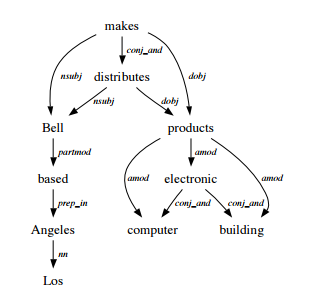
\includegraphics[scale=0.8]{dependency_tree}\end{center}
\caption[Strom vzťahov]{Strom vzťahov}\label{fig:dependency_tree}
\end{figure}

V tomto orientovanom stromovom grafe jednotlivé slová vety predstavujú vrcholy, pričom prechody medzi vrcholmi, hrany, reprezentujú vzťahy medzi nimi.

Ďalšia reprezentácia závislostí zapisuje vzťahy priamo do vety. Na obrázku \fullref{fig:dependencies_in_sentence} vidíme, že medzi slovami \textit{She} a \textit{looks} je vzťah \textbf{nsubj} - nominal subject, medzi \textit{looks} a \textit{beautiful} je vzťah \textbf{acomp} - adjectival complement, a v neposlednom rade medzi slovami \textit{very} a \textit{beautiful} je vzťah \textbf{advmod} - adverb modifier~\cite{StanfordDepManual}.

\begin{figure}[H]
\begin{center}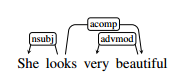
\includegraphics[scale=0.8]{dependencies_in_sentence}\end{center}
\caption[Vzťahy vo vete]{Vzťahy vo vete}\label{fig:dependencies_in_sentence}
\end{figure}

Celá závislosť sa skladá primárne z nadradeného tokenu, podradeného tokenu a vzťahu medzi nimi. Na obrázku~\fullref{fig:dependencies_in_sentence} vidno, okrem iných aj závislosť, ktorej nadradený token je slovo \textit{looks}, podradený token je slovo \textit{She} a vzťah je \textit{nsubj}.

%
% Extrakcia informácií
%
\ifthenelse {\boolean{bachelor}}
{
	%\subsection{Subsection}
	\subsubsection{Extrakcia informácií}
}
{
	%\section{Subsection}
	\subsubsection{Extrakcia informácií}
}
\label{subsubsec:information_extraction}
Systémy a aplikácie zamerané na extrakciu informácií vyhľadávajú a extrahujú informácie z textov, článkov a dokumentov, pričom reagujú na používateľove informačné potreby. Výstup z takýchto systémov a aplikácií nepozostáva iba zo zoznamu kľúčových slov, ktoré by sa dali pokladať za extrahované informácie, ale naopak sú v tvare preddefinovaných šablón~\cite{Preeti}.

Extrakcia informácií využíva niekoľko z hlavných úloh spracovania prirodzeného jazyka. Sú to \textit{značkovanie slovných druhov}, \textit{rozpoznávanie názvoslovných entít}, a ďalšie~\cite{Preeti}. Tieto a aj ostatné úlohy spracovania prirodzeného jazyka sú podrobnejšie opísané v sekcii \fullref{subsec:tasksofnlp}.

Výber informácií a extrakcia informácií spolu úzko súvisia, ale sú to dve rozdielne využitia spracovania prirodzeného jazyka. Prvé spomínané využitie slúži na vyhľadávanie relevantných zdrojov informácií v databázach textov, článkov a dokumentov podľa používateľových potrieb. Na vyhľadaných zdrojoch následne prebehne extrakcia informácií. 

%My sa pri spracovaní textov zameriame hlavne na extrakciu informácií, aby sme dokázali z učebného textu extrahovať relevantné informácie pre študenta, a tým získali poznámky.

%
% Nástroje na spracovanie prirodzeného jazyka
%
\ifthenelse {\boolean{bachelor}}
{
	%\subsection{Subsection}
	\subsection{Nástroje na spracovanie prirodzeného jazyka}
}
{
	%\section{Subsection}
	\section{Nástroje na spracovanie prirodzeného jazyka}
}
\label{subsec:nlp_nastroje}
V súčastnosti je vyvinutých, alebo sú vo vývoji, viaceré nástroje, ktoré sa dajú použiť pri spracovávaní prirodzeného jazyka. Vývoj takýchto nástrojov je podporovaný na známych univerzitách ako sú napríklad Princeton, Stanford alebo Camridge, ale aj mimo univerzít napríklad v Google. 

%
% WordNet
%
\ifthenelse {\boolean{bachelor}}
{
	%\subsection{Subsection}
	\subsubsection{WordNet}
}
{
	%\section{Subsection}
	\subsection{WordNet}
}
\label{subsubsec:wordnet}
WordNet\footnote{www.wordnet.princeton.edu} je databáza anglických slov vyvíjaná na Princetonskej univerzite. Databáza obsahuje podstatné mena, prídavné mená, slovesá a príslovky, ktoré sú zatriedené do synonymických sád, synsetov.

Slová do synetov sú zaraďované podľa významu. To znamená, že slová auto a automobil, ktoré sú pre svoj význam zameniteľné vo vete, sa zaraďujú do rovnakého synsetu. WordNet v súčasnosti (r. 2015) obsahuje 117 000 synsetov. Každý z nich obsahuje aj krátku ukážku použitia slova.

Vo WordNet sa nachádzajú aj vzťahy medzi slovami v zmysle nadradenosti. To znamená, že \textit{stolička} je nábytok a nábytok je fyzická vec a takto to pokračuje až po najvyššie slovo, od ktorého ,,dedia'' všetky - entita (viď. obrázok \fullref{fig:wordnet_relations}. Okrem vzťahu nadradenosti WordNet obsahuje aj vzťah zloženia. Stolička sa skladá z operadla a nôh. Toto zloženie je typické len pre konkrétne slovo a neprenáša sa hore stromom nadradenosti,   lebo pre stoličku je typické, že sa skladá z operadla a nôh, ale to už nie je typické pre nábytok.
Prídavné mená obsahujú aj vzťah antonymity, takže slovo \textit{suchý} bude prepojené so slovom \textit{mokrý} ako so svojím antonymom.

Tento nástroj je dostupný vo webovej verzií (viď. obrázok \fullref{fig:wordnet_search}), ale ponúka aj stiahnutie jeho databázových súborov, ktoré sa po splnení licenčných požiadaviek dajú využívať v projektoch.

\begin{figure}[H]
\begin{center}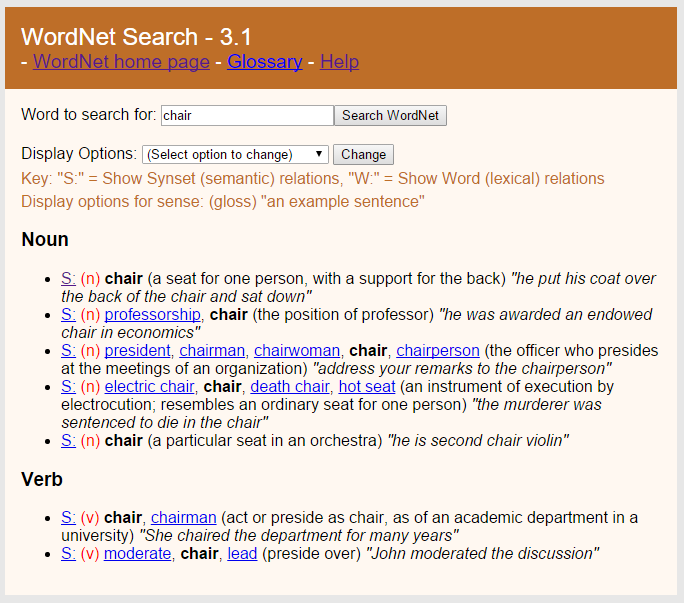
\includegraphics[scale=0.48]{wordnet_search}\end{center}
\caption[Webové rozhranie]{Webové rozhranie (Wordnet)}\label{fig:wordnet_search}
\end{figure}

\begin{figure}[H]
\begin{center}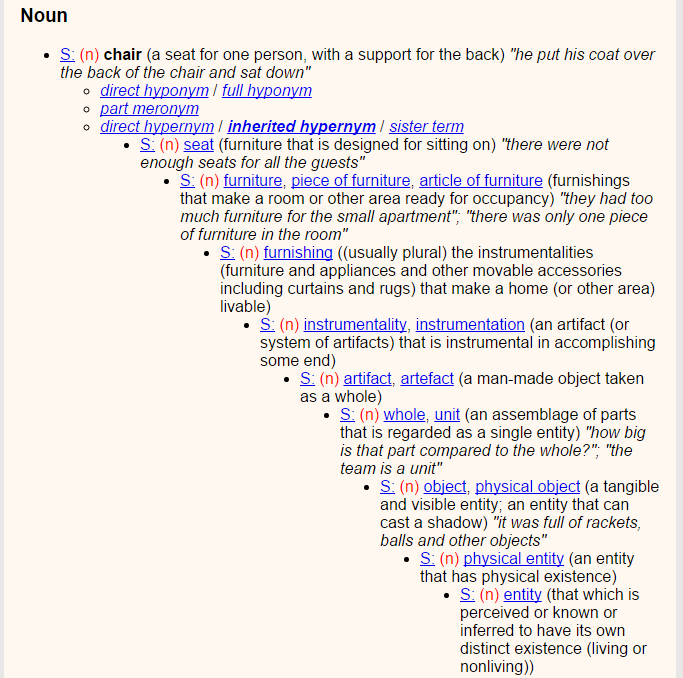
\includegraphics[scale=0.48]{wordnet_search_relations}\end{center}
\caption[Nadradenosť slov]{Nadradenosť slov (Wordnet)}\label{fig:wordnet_relations}
\end{figure}

%
% StanfordNLP
%
\ifthenelse {\boolean{bachelor}}
{
	%\subsection{Subsection}
	\subsubsection{StanfordNLP}
}
{
	%\section{Subsection}
	\subsection{StanfordNLP}
}
\label{subsubsec:stanfordnlp}
Nástroj StanfordNLP\footnote{www.nlp.stanford.edu} je vyvíjaný na Stanfordskej univerzite. Skladá sa z niekoľkých softvérov, ktoré sa zameriavajú na úlohy spracovania prirodzeného jazyka popísané v sekcií \fullref{subsec:tasksofnlp}. Sú to softvéry \textit{Stanford Parser}, \textit{Stanford POS Tagger}, \textit{Stanford EnglishTokenizer}, \textit{Stanford Relation Extractor} a mnoho ďalších. \textit{Stanford CoreNLP} zahŕňa viacero zo spomenutých softvérov.

Nástroje StanfordNLP sú implementované v Jave, ale dostupné aj v iných programovacích jazykoch ako C\#, PHP alebo Python.

Dostupné je aj online webové demo. Na obrázku \fullref{fig:stanfordnlp_online_demo} vidno výstupy z nástrojov ponúkaných balíkom StanfordNLP pre jednoduchý vstupný text skladajúci sa z jednej vety ,,Martin Nemček is a student at Slovak University of Technology in Bratislava.''.

\begin{figure}[H]
\begin{center}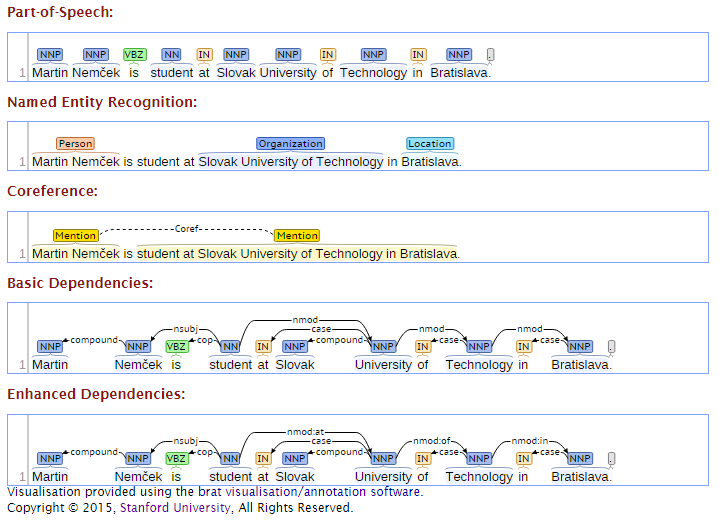
\includegraphics[scale=0.52]{stanfordnlp_online}\end{center}
\caption[StanfordNLP online demo]{StanfordNLP online demo}\label{fig:stanfordnlp_online_demo}
\end{figure}

%
% CambridgeAPI
%
\ifthenelse {\boolean{bachelor}}
{
	%\subsection{Subsection}
	\subsubsection{CambridgeAPI}
}
{
	%\section{Subsection}
	\subsection{CambridgeAPI}
}
\label{subsubsec:cambridgeapi}
CambridgeAPI\footnote{www.dictionary-api.cambridge.org} je nástroj vytvorený na Cambridge univerzite. Umožňuje prístup k viacerým slovníkom. Momentálne (r. 2015) tento nástroj ponúka prístup k pätnástim prekladovým slovníkom, ako napríklad anglicko-čínsky, anglicko-ruský, anglicko-arabský, anglicko-japonský a ďalšie. Všetky prekladové slovníky majú primárny jazyk angličtinu. Slovenčinu v súčastnosti nepodporuje.

Spomínaný nástroj funguje na princípe dopytovania pomocou HTTP protokolu. Na obdržanie korektnej odpovede je potrebné mať osobný API kľúč. Ten sa dá získať kontaktovaním správcov CambridgeAPI.

%
% Google Ngram
%
\ifthenelse {\boolean{bachelor}}
{
	%\subsection{Subsection}
	\subsubsection{Google Ngram}
}
{
	%\section{Subsection}
	\subsection{Google Ngram}
}
\label{subsubsec:googlengram}
Google Ngram\footnote{www.books.google.com/ngrams} je postavený na ďalšom softvéri od spoločnosti Google, Google Books. V knihách, napísaných od roku 1500 až do súčastnosti, vyhľadáva výskyty n-gramov. Podporuje len niektoré jazyky, ako angličtina, francúzština, ruština alebo čínština. Na vyhľadávanie v knihách využíva optické rozpoznávanie textu, pričom dokáže spracovať aj regulárne výrazy, avšak tie môžu byť použité iba ako náhrada celého slova, ale nie uprostred slova. Regulárny výraz \textit{,,* Einstein''} spracuje, pričom \textit{,,Albert Einste*n''} nie.

N-gram je podľa oxfordského slovníka\footnote{http://www.oxforddictionaries.com/} definovaný ako postupnosť \textit{n} za sebou idúcich slov alebo znakov. \textit{Martin} je n-gram veľkosti jedna, teda 1-gram alebo unigram. \textit{Martin Nemček} je n-gram veľkosti dva, 2-gram alebo bigram a tak ďalej, pričom \textit{n} môže byť ľubovoľné kladné, celé číslo.

Google Ngram Viewer poskytuje vizualizáciu vyhľadaných dát a je dostupný vo webovom rozhraní. Na obrázku \fullref{fig:googlengram_visualization} vidno vizualizáciu výskytu mien \textit{Albert Einstein, Sherlock Holmes, Frankenstein} v knihách od roku 1800 do roku 2000.

\begin{figure}[H]
\begin{center}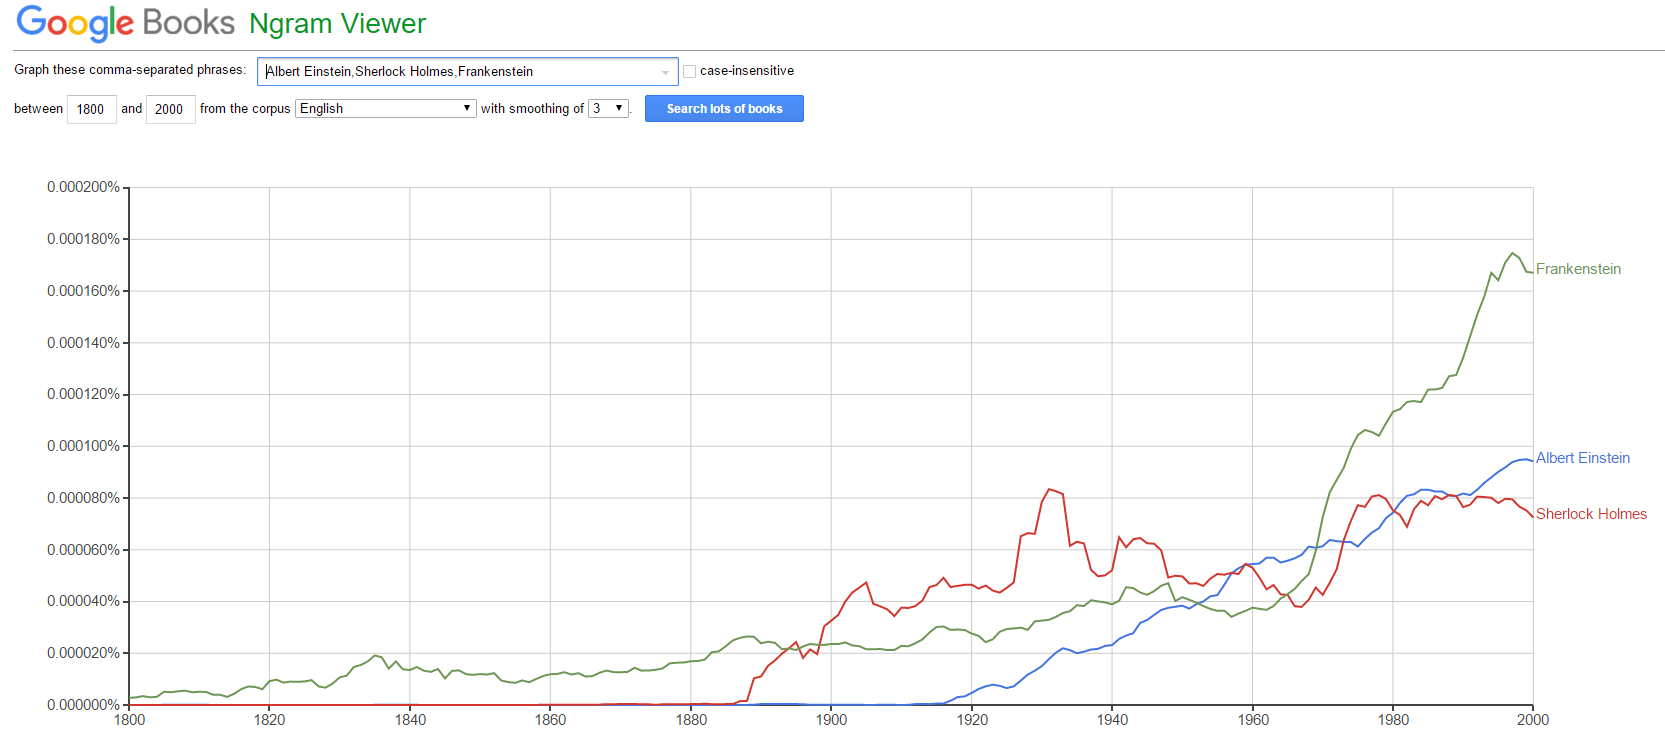
\includegraphics[scale=0.30]{googlengram_visualization}\end{center}
\caption[Google Ngram Viewer]{Google Ngram Viewer}\label{fig:googlengram_visualization}
\end{figure}

Tento nástroj okrem iného ponúka aj surové (angl. raw) dáta na stiahnutie.

%
% AlchemyAPI
%
\ifthenelse {\boolean{bachelor}}
{
	%\subsection{Subsection}
	\subsubsection{AlchemyAPI}
}
{
	%\section{Subsection}
	\subsection{AlchemyAPI}
}
\label{subsubsec:alchemyapi}
AlchemiAPI\footnote{www.alchemyapi.com} je súbor dvanástich nástrojov, z ktorých sú niektoré zamerané na úlohy spracovania prirodzeného jazyka popísané v sekcií \fullref{subsec:tasksofnlp}, ako napríklad extrakcia entít, extrakcia kľúčových slov, extrakcia vzťahov, ale aj iné zaujímave funkcie, napríklad extrakcia autora z textu.

Na používanie tohto nástroja je potrebná registrácia pre obdržanie API kľúču. S týmto kľúčom je tisíc dopytov denne zdarma. Dostupnosť v programovacích jazykoch je široká. Ponúka knižnicu v deviatich najpoužívanejších programovacích jazykoch.

Pre AlchemyAPI je dostupné aj online webové demo, viď obrázok \fullref{fig:alchemyapi_visualization}, kde je vidno širokú ponuku, obsiahnutú v tomto nástroji.

\begin{figure}[H]
\begin{center}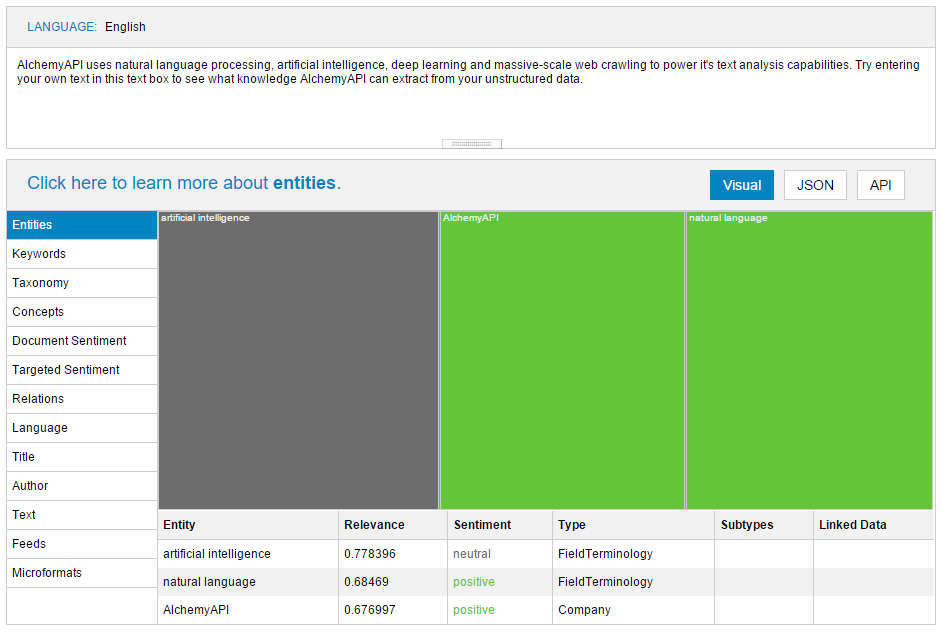
\includegraphics[scale=0.48]{alchemyapi_visualization}\end{center}
\caption[AlchemyAPI online demo]{AlchemyAPI online demo}\label{fig:alchemyapi_visualization}
\end{figure}

Dáta sú vo formáte JSON a okrem spracovania prirodzeného jazyka AlchemyAPI ponúka aj nástroje na extrahovanie obsahu z obrázku alebo rozpoznávanie tvárí na obrázkoch.

%
% Zhrnutie
%
\ifthenelse {\boolean{bachelor}}
{
	%\subsection{Subsection}
	\subsection{Zhrnutie}
}
{
	%\section{Subsection}
	\section{Zhrnutie}
}
\label{subsec:analysis:zhrnutie}

Dummy text..